\subsection{Simple example for more than one genotype per infection}\label{ex:multiple_genos}

\paragraph{Observed and phased alleles} In a simple example two and one alleles are observed at a single marker genotyped in an incident and single recurrent infection, respectively. We assume the most parsimonious explanation of the data: the number of genotypes in the first and second infections are two and one, respectively. There is no-longer a one-to-one mapping between genotypes and infections over time. Instead, there are two possible allele assignments: 
\begin{equation*}
    \bm{y} = \begin{blockarray}{cc}\\
    j=1\\
        \begin{block}{(c)c}
        \{A,T\}  & t=0\\
        \{T\} & t=1\\
        \end{block}
        \end{blockarray},
        \hspace{1cm}
    \bm{a}_\RN{1} = \begin{blockarray}{cc}\\
    j=1\\
        \begin{block}{(c)c}
        A & i=1, \; t=0\\
        T & i=2, \; t=0\\
        T & i=3, \; t=1\\
        \end{block}
        \end{blockarray},\hspace{1cm}
    \bm{a}_\RN{2} = \begin{blockarray}{cc}\\
    j=1\\
        \begin{block}{(c)c}
        T & i=1, \; t=0\\
        A & i=2, \; t=0\\
        T & i=3, \; t=1\\
        \end{block}
        \end{blockarray}.
\end{equation*}
Since $\bm{a}_\RN{1}$ and $\bm{a}_\RN{2}$ are equivalent up to a swap between the two genotypes in the first episode, we have $s\in\{L,I,C\}$ that $\mathbb{P}(\bm{y}|s) = 2\mathbb{P}(\bm{a}_\RN{1}|s)$.

\paragraph{Relationship graphs and IBD partitions} There are nine relationship graphs (a subset of those in example \ref{ex:multiple_recurs_het} because clonal relationships within infections are disallowed) to sum over and five IBD partitions (the same as those in example \ref{ex:multiple_recurs_het}), corresponding to the same five IBD graphs as follows.

\begin{center}
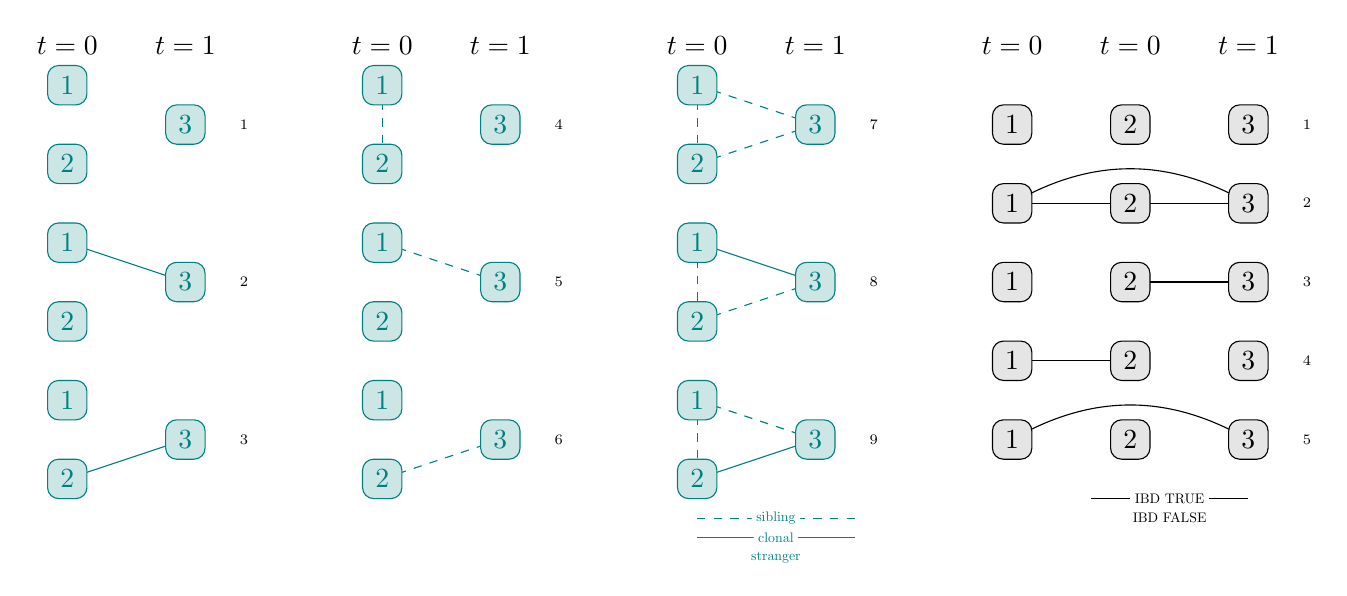
\begin{tikzpicture}
    \tikzstyle{geno} = [draw, rectangle, rounded corners, minimum height=0.5cm, minimum width=0.5cm, color=teal, fill=teal!20]
    \tikzstyle{ibd} = [draw, rectangle, rounded corners, minimum height=0.5cm, minimum width=0.5cm, fill=gray!20]
    
    \node at (0,1) {$t=0$};
    \node at (1.5,1) {$t=1$};
    \node at (4,1) {$t=0$};
    \node at (5.5,1) {$t=1$};
    \node at (8,1) {$t=0$};
    \node at (9.5,1) {$t=1$};
    \node at (12,1) {$t=0$};
    \node at (13.5,1) {$t=0$};
    \node at (15,1) {$t=1$};
    
    \node[scale = 0.75] at (2.25,0) {$\rg_\RN{1}$};
    \node[scale = 0.75] at (2.25,-2) {$\rg_\RN{2}$};
    \node[scale = 0.75] at (2.25,-4) {$\rg_\RN{3}$}; 
    \node[scale = 0.75] at (6.25,0) {$\rg_\RN{4}$};
    \node[scale = 0.75] at (6.25,-2) {$\rg_\RN{5}$};
    \node[scale = 0.75] at (6.25,-4) {$\rg_\RN{6}$}; 
    \node[scale = 0.75] at (10.25,0) {$\rg_\RN{7}$};
    \node[scale = 0.75] at (10.25,-2) {$\rg_\RN{8}$};
    \node[scale = 0.75] at (10.25,-4) {$\rg_\RN{9}$}; 
    \node[scale = 0.75] at (15.75,0) {$\ip_\RN{1}$};
    \node[scale = 0.75] at (15.75,-1) {$\ip_\RN{2}$};
    \node[scale = 0.75] at (15.75,-2) {$\ip_\RN{3}$}; 
    \node[scale = 0.75] at (15.75,-3) {$\ip_\RN{4}$};
    \node[scale = 0.75] at (15.75,-4) {$\ip_\RN{5}$};
 
    % Graph 1
    \node[geno] at (0,0.5) {$1$};
    \node[geno] at (0,-0.5) {$2$};
    \node[geno] at (1.5,0) {$3$}; 
    
    % Graph 2
    \draw[geno](0,-1.5) -- (1.5,-2);
    \node[geno] at (0,-1.5) {$1$};
    \node[geno] at (0,-2.5) {$2$};
    \node[geno] at (1.5,-2) {$3$}; 
    
    % Graph 3
    \draw[geno] (0,-4.5) -- (1.5,-4);
    \node[geno] at (0,-3.5) {$1$};
    \node[geno] at (0,-4.5) {$2$};
    \node[geno] at (1.5,-4) {$3$}; 
    
    % Graph 4
    \draw[geno, dashed](4,0.5) -- (4,-0.5);
    \node[geno] at (4,0.5) {$1$};
    \node[geno] at (4,-0.5) {$2$};
    \node[geno] at (5.5,0) {$3$}; 
    
    % Graph 5
    \draw[geno, dashed](4,-1.5) -- (5.5,-2);
    \node[geno] at (4,-1.5) {$1$};
    \node[geno] at (4,-2.5) {$2$};
    \node[geno] at (5.5,-2) {$3$}; 
    
    % Graph 6
    \draw[geno, dashed](4,-4.5) -- (5.5,-4);
    \node[geno] at (4,-3.5) {$1$};
    \node[geno] at (4,-4.5) {$2$};
    \node[geno] at (5.5,-4) {$3$}; 
    
    % Graph 7
    \draw[geno, dashed](8,0.5) -- (8,-0.5);
    \draw[geno, dashed](9.5,0) -- (8,0.5);
    \draw[geno, dashed](9.5,0) -- (8,-0.5);
    \node[geno] at (8,0.5) {$1$};
    \node[geno] at (8,-0.5) {$2$};
    \node[geno] at (9.5,0) {$3$}; 
    
    % Graph 8
    \draw[geno](8,-1.5) -- (9.5,-2);
    \draw[geno, dashed](9.5,-2) -- (8,-2.5);
    \draw[geno, dashed](8,-1.5) -- (8,-2.5);
    \node[geno] at (8,-1.5) {$1$};
    \node[geno] at (8,-2.5) {$2$};
    \node[geno] at (9.5,-2) {$3$}; 
    
    % Graph 9
    \draw[geno](8,-4.5) -- (9.5,-4);
    \draw[geno, dashed](9.5,-4) -- (8,-3.5);
    \draw[geno, dashed](8,-3.5) -- (8,-4.5);
    \node[geno] at (8,-3.5) {$1$};
    \node[geno] at (8,-4.5) {$2$};
    \node[geno] at (9.5,-4) {$3$}; 
    
    % Graph 1
    \node[ibd] at (12,0) {$1$};
    \node[ibd] at (13.5,0) {$2$};
    \node[ibd] at (15,0) {$3$}; 
    
    % Graph 2
    \path[bend left] (12,-1) edge (15,-1);
    \draw (12,-1) -- (13.5,-1);
    \draw (13.5,-1) -- (15,-1);
    \node[ibd] at (12,-1) {$1$};
    \node[ibd] at (13.5,-1) {$2$};
    \node[ibd] at (15,-1) {$3$}; 
    
    % Graph 3
    \draw (13.5,-2) -- (15,-2);
    \node[ibd] at (12,-2) {$1$};
    \node[ibd] at (13.5,-2) {$2$};
    \node[ibd] at (15,-2) {$3$}; 
    
    % Graph 4
    \draw (12,-3) -- (13.5,-3);
    \node[ibd] at (12,-3) {$1$};
    \node[ibd] at (13.5,-3) {$2$};
    \node[ibd] at (15,-3) {$3$}; 
    
    % Graph 5
    \path[bend left] (12,-4) edge (15,-4);
    \node[ibd] at (12,-4) {$1$};
    \node[ibd] at (13.5,-4) {$2$};
    \node[ibd] at (15,-4) {$3$}; 
    
    % Legend
    \draw[dashed, geno] (8,-5) -- (10,-5) 
    node[scale=0.5, midway, fill=white]{sibling};
    \draw[geno] (8,-5.25) -- (10,-5.25) 
    node[scale=0.5, midway, fill=white]{clonal};
    \path (8,-5.5) -- (10,-5.5) 
    node[scale=0.5, midway, fill=white, text = teal]{stranger};
    \draw (13,-4.75) -- (15,-4.75) 
    node[scale=0.5, midway, fill=white]{IBD TRUE};
    \path (13,-5) -- (15,-5) 
    node[scale=0.5, midway, fill=white]{IBD FALSE};
\end{tikzpicture}
\end{center}

\paragraph{Likelihood} Remembering that in linear algebra $(CBA)^T = (A^TB^TC^T)$, 
\begin{align*}
&\mathbb{P}(\bm{y}|s)\forall s\in\{L,I,C\} = 
2 \underbrace{ 
    \begin{blockarray}{cl}
    \bm{a}_\RN{1} \\
    \begin{block}{(c)l}
    \sfrac{5}{18}f(A)f(T)^2 + \sfrac{1}{4}f(A)f(T) & L \\
    \sfrac{3}{4}f(A)f(T)^2 & I \\ 
    \sfrac{3}{8} f(A)f(T) & C \\ 
    \end{block}
    \end{blockarray}
    }_{\mathclap{\mathbb{P}(\bm{a}_\RN{1}|\bm{s})\forall\bm{s}\in\{L,I,C\}}},
    \\
&=2 \underbrace{
    \begin{blockarray}{cccccccccl}
        \rg_\RN{1} & \rg_\RN{2} & \rg_\RN{3} & 
        \rg_\RN{4} & \rg_\RN{5} & \rg_\RN{6} &
        \rg_\RN{7} & \rg_\RN{8} & \rg_\RN{9}\\
        \begin{block}{(ccccccccc)l}
          \sfrac{1}{9} & \sfrac{1}{9} & \sfrac{1}{9} & 
          \sfrac{1}{9} & \sfrac{1}{9} & \sfrac{1}{9} &
          \sfrac{1}{9} & \sfrac{1}{9} & \sfrac{1}{9} 
          & L \\
          \sfrac{1}{2} &0&0 & \sfrac{1}{2} &0&0&0&0&0 
          & I \\
          0&\sfrac{1}{4}&\sfrac{1}{4}&0&0&0&0&
          \sfrac{1}{4}&\sfrac{1}{4}
          & C \\
        \end{block}
        \end{blockarray}
}_{\mathclap{\mathbb{P}(\rg|s)\forall\rg\in\RG,s\in\{L,I,C\}}} 
\times \quad
\underbrace{ 
    \begin{blockarray}{cl}
    {\bm{a}_\RN{1}}_{\cdot 1} \\
    \begin{block}{(c)l}
    f(A)f(T)^2 & \rg_\RN{1} \\
    0 & \rg_\RN{2} \\ 
    f(A)f(T) & \rg_\RN{3} \\ 
    \sfrac{1}{2}f(A)f(T)^2 & \rg_\RN{4} \\ 
    \sfrac{1}{2}f(A)f(T)^2 & \rg_\RN{5} \\
    \sfrac{1}{2}f(A)f(T)(f(T)+1) &\rg_\RN{6} \\
    \sfrac{1}{4}f(A)f(T) & \rg_\RN{7} \\
    0 &\rg_\RN{8}\\
    \sfrac{1}{2}f(A)f(T) &\rg_\RN{9} \\
    \end{block}
    \end{blockarray}
    }_{\mathclap{\mathbb{P}({\bm{a}_\RN{1}}_{\cdot j}|\rg)\forall{\bm{a}_\RN{1}}_{\cdot j}\in\bm{a}_\RN{1},\rg\in\RG}},
\\
&=2 \underbrace{
    \begin{blockarray}{cccccccccl}
        \rg_\RN{1} & \rg_\RN{2} & \rg_\RN{3} & 
        \rg_\RN{4} & \rg_\RN{5} & \rg_\RN{6} &
        \rg_\RN{7} & \rg_\RN{8} & \rg_\RN{9}\\
        \begin{block}{(ccccccccc)l}
          \sfrac{1}{9} & \sfrac{1}{9} & \sfrac{1}{9} & 
          \sfrac{1}{9} & \sfrac{1}{9} & \sfrac{1}{9} &
          \sfrac{1}{9} & \sfrac{1}{9} & \sfrac{1}{9} 
          & L \\
          \sfrac{1}{2} &0&0 & \sfrac{1}{2} &0&0&0&0&0 
          & I \\
          0&\sfrac{1}{4}&\sfrac{1}{4}&0&0&0&0&
          \sfrac{1}{4}&\sfrac{1}{4}
          & C \\
        \end{block}
        \end{blockarray}
}_{\mathclap{\mathbb{P}(\rg|s)\forall\rg\in\RG,s\in\{L,I,C\}}} 
\times \\
&\underbrace{ 
    \begin{blockarray}{cccccl}
    \ip_\RN{1} & \ip_\RN{2} & \ip_\RN{3} & 
    \ip_\RN{4} & \ip_\RN{5} \\
    \begin{block}{(ccccc)l}
    1&0&0&0&0&\rg_\RN{1} \\
    0&0&0&0&1&\rg_\RN{2} \\
    0&0&1&0&0&\rg_\RN{3}  \\
    \sfrac{1}{2}&0&0&\sfrac{1}{2}&0&\rg_\RN{4} \\
    \sfrac{1}{2}&0&0&0&\sfrac{1}{2}&\rg_\RN{5} \\
    \sfrac{1}{2}&0&\sfrac{1}{2}&0&0&\rg_\RN{6} \\
    0&\sfrac{1}{4}&\sfrac{1}{4}&\sfrac{1}{4}&\sfrac{1}{4}&\rg_\RN{7} \\
    0&\sfrac{1}{2}&0&0&\sfrac{1}{2}&\rg_\RN{8} \\
    0&\sfrac{1}{2}&\sfrac{1}{2}&0&0&\rg_\RN{9} \\
    \end{block}
    \end{blockarray}
    }_{\mathclap{\mathbb{P}(\ip|\rg)\forall\ip\in\IP,\rg\in\RG}} 
    \times \quad
    \underbrace{ 
    \begin{blockarray}{cl}
    {\bm{a}_\RN{1}}_{\cdot 1} \\
    \begin{block}{(c)l}
    f(A)f(T)^2 & \ip_\RN{1} \\
    0 & \ip_\RN{2} \\ 
    f(A)f(T) & \ip_\RN{3} \\ 
    0 & \ip_\RN{4} \\ 
    0 & \ip_\RN{5} \\
    \end{block}
    \end{blockarray}
    }_{\mathclap{\mathbb{P}({\bm{a}_\RN{1}}_{\cdot j}|\ip)\forall{\bm{a}_\RN{1}}_{\cdot j}\in\bm{a}_\RN{1},\ip\in\IP}}.
\end{align*}

\noindent
The prefactor of 2 corresponds to $\A$ consisting of an equivalence class of 2 allele assignments. Note that if the data for the incident infection and the recurrence were reversed, e.g. if $\bm{y}_{t=0} = \{T\}$ and $\bm{y}_{t=1} = \{A,T\}$, the posterior probability of recrudescence would be zero because recrudescences must have the same or fewer genotypes than the directly preceding infection. 

\paragraph{Posterior} For a uniform prior on $s\in\{L,I,C\}$, $\mathbb{P}(\bm{y}) = \tfrac{1}{3}\Big(\tfrac{37}{36}f(A)f(T)^2 + \tfrac{5}{8}f(A)f(T)\Big)$ and 
\begin{equation*}
    \mathbb{P}(s_1 | \bm{y}) \forall s_1\in\{L,I,C\} 
    =
    {\underbrace{\Big(\tfrac{37}{108}f(A)f(T)^2 + \tfrac{5}{24}f(A)f(T)\Big)
    }_{\mathclap{\mathbb{P}(\bm{y})}}}^{-1} \times \tfrac{1}{3} \times 
    \underbrace{ 
    \begin{blockarray}{cl}
    \begin{block}{(c)l}
    \sfrac{5}{18}f(A)f(T)^2 + \sfrac{1}{4}f(A)f(T) & L \\
    \sfrac{3}{4}f(A)f(T)^2 & I \\ 
    \sfrac{3}{8} f(A)f(T) & C \\ 
    \end{block}
    \end{blockarray}
    }_{\mathclap{\mathbb{P}(\bm{y}|\bm{s})\forall\bm{s}\in\{L,I,C\}}},
\end{equation*}

\subsection{Simple zoomed-in example for six genotypes}\label{ex:cells}

\paragraph{Observed and phased alleles} Suppose the observed alleles suggest there are $n>3$ genotypes, e.g., 
\begin{align*}
    \bm{y} = 
    \begin{blockarray}{cl}\\
    j=1\\
    \begin{block}{(c)l}
    \{A,T,C\} & t=0 \\
    \{A,T\} & t=1 \\
    \{A\} & t=2 \\
    \end{block}
    \end{blockarray},
    \hspace{1cm}
    \bm{a} = 
    \begin{blockarray}{cl}\\
    j=1 \\
    \begin{block}{(c)l}
    A & i=1 \\
    T & i=2 \\
    C & i=3 \\
    A & i=4 \\
    T & i=5 \\
    A & i=6 \\
    \end{block}
    \end{blockarray}.
\end{align*}

\paragraph{IBD partitions}
For $n=6$, there are 203 IBD partitions in $\IP$. Three examples, depicted below as graphs, are:  
\begin{align*}
    \ip_\RN{1} &= \{\{\{1,4,6\},\{2,5\},\{3\}\}, \\
    \ip_\RN{2} &= \{\{1,2\},\{3,5\},\{4,6\}\}, \\
    \ip_\RN{3} &= \{\{1\},\{2\},\{3\},\{4\},\{5\},\{6\}\}. \\
\end{align*}
 
\begin{center}
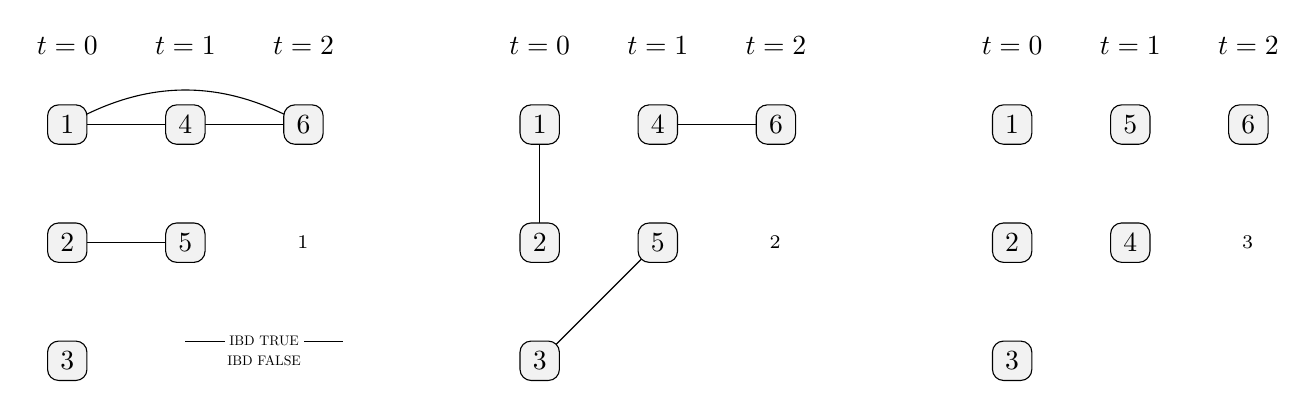
\begin{tikzpicture}
    \tikzstyle{ibd} = [draw, rectangle, rounded corners, minimum height=0.5cm, minimum width=0.5cm, fill = gray!10]
    
    \node at (0,1) {$t=0$};
    \node at (1.5,1) {$t=1$};
    \node at (3,1) {$t=2$}; 
    \node at (6,1) {$t=0$};
    \node at (7.5,1) {$t=1$};
    \node at (9,1) {$t=2$}; 
    \node at (12,1) {$t=0$};
    \node at (13.5,1) {$t=1$};
    \node at (15,1) {$t=2$}; 
   
    % IBD partition
    \path[ibd, bend left] (0,0) edge (3,0);
    \draw[ibd] (0,0) -- (1.5,0);
    \draw[ibd] (1.5,0) -- (3,0);
    \draw[ibd] (0,-1.5) -- (1.5,-1.5);
    \node[ibd] at (0,0) {$1$};
    \node[ibd] at (0,-1.5) {$2$};
    \node[ibd] at (0,-3) {$3$};
    \node[ibd] at (1.5,0) {$4$};
    \node[ibd] at (1.5,-1.5) {$5$};
    \node[ibd] at (3,0) {$6$};
    \node at (3,-1.5) {$\ip_\RN{1}$}; 
    
    % IBD partition
    \draw[ibd] (6,0) -- (6,-1.5);
    \draw[ibd] (6,-3) -- (7.5,-1.5);
    \draw[ibd] (7.5,0) -- (9,0);
    \node[ibd] at (6,0) {$1$};
    \node[ibd] at (6,-1.5) {$2$};
    \node[ibd] at (6,-3) {$3$};
    \node[ibd] at (7.5,0) {$4$};
    \node[ibd] at (7.5,-1.5) {$5$};
    \node[ibd] at (9,0) {$6$}; 
    \node at (9,-1.5) {$\ip_\RN{2}$}; 
    
    % IBD partition
    \node[ibd] at (12,0) {$1$};
    \node[ibd] at (12,-1.5) {$2$};
    \node[ibd] at (12,-3) {$3$};
    \node[ibd] at (13.5,-1.5) {$4$};
    \node[ibd] at (13.5,0) {$5$};
    \node[ibd] at (15,0) {$6$}; 
    \node at (15,-1.5) {$\ip_\RN{3}$}; 

    % Legend
    \draw (1.5,-2.75) -- (3.5,-2.75) 
    node[scale=0.5, midway, fill=white]{IBD TRUE};
    \path (1.5,-3) -- (3.5,-3) 
    node[scale=0.5, midway, fill=white]{IBD FALSE};
\end{tikzpicture}
\end{center}

\begin{align*}
    \mathbb{P}({\bm{a}}_{\cdot 1} | \ip_\RN{1}) 
    &= 
    \mathbb{P}({\bm{a}}_{\{1,4,6\} 1} | \{1,4,6 \}) \times
    \mathbb{P}({\bm{a}}_{\{2,5\} 1} | \{2,5 \}) \times
    \mathbb{P}(a_{3 1} | \{3\}), \\
    &= f(A_1) \times f(T_1) \times f(C_1)
    .\\
    % =====
    \mathbb{P}({\bm{a}}_{\cdot 1} | \ip_\RN{2}) 
    &= 
    \mathbb{P}({\bm{a}}_{\{12\} 1} | \{1,2 \}) \times
    \mathbb{P}({\bm{a}}_{\{3,5\} 1} | \{3,5 \}) \times
    \mathbb{P}({\bm{a}}_{\{4,6\} 1} | \{4,6\}), \\
    &= 0 \times 0 \times f(A_1)
    .\\
    \mathbb{P}({\bm{a}}_{\cdot 1} | \ip_\RN{3}) 
    &= 
    \mathbb{P}(a_{11} | \{1\}) \times
    \mathbb{P}(a_{21} | \{2\}) \times
    \mathbb{P}(a_{31} | \{3\}) \times
    \mathbb{P}(a_{41} | \{4\}) \times
    \mathbb{P}(a_{51} | \{5\}) \times
    \mathbb{P}(a_{61} | \{6\}), \\
    &= f(A)^3 \times f(T)^2 \times f(C).
\end{align*} 